\setcounter{chapter}{1} 

\chapter{Lightning}\label{ch:lightning}
Observation of lightning is a  natural part of human history, from early man believing it to be caused by the wrath of deities, to the modern storm chaser utilizing radar observations of precipitation to get the best view of a storm. The scientific study of lightning, on the other hand, is relatively new. The first steps towards systematic study were the experiments performed by Benjamin Franklin, along with the development of the theory of electromagnetism. Only in the last century have we acquired the means to thoroughly investigate the electrical and meteorological mechanisms resulting in a thunderstorm. This is due to both more available measurements and better physical understanding. The measurements are made possible by aircraft being able to fly through storm clouds providing in-situ observations, and satellite imagery providing a view into the vertical composition and structure of clouds.

This chapter briefly explains cloud creation, cloud electrification and lightning, and finally what is known about what separates \acrlong{htl} and \acrlong{fwtl} from natural lightning.

\section{Convection and cloud creation}

Lightning occurs in storm clouds, and therefore an explanation of cloud creation mechanisms is necessary to understand why lightning occurs. One of the key components to cloud creation is an unstable atmosphere: an atmosphere where temperature decreases with height. Instability can be understood by recognizing that warm air is less dense than cold air, and thus buoyant in the colder surrounding air. When air rises, less pressure is exerted on it, since the atmosphere is densest at the surface. This lower pressure causes work to be done by the rising air, to expand to a new equilibrium. If the air rises fast enough for the expansion to be adiabatic, this work leads to a cooling of the air mass. This cooling slows the vertical movement due to less buoyancy.

However, if moisture is present at the surface, water vapor will be displaced upwards by this vertical movement. When the air mass is cooled by the expansion, the saturation vapor pressure decreases. Lower saturation vapor pressure favours more water in the condensed phase, either as ice or water particles. Condensation of water vapor heats the ascending air, which causes more vertical movement. Thus, a dry atmosphere is inherently more stable than a humid atmosphere, as the lack of condensation would lead to equilibrium due to adiabatic cooling alone.

If temperatures are sufficiently low ($\leq 0 ^{\circ} C$), the liquid water may freeze to ice crystals. The uncertainty here is due to the heat released when a crystalline surface is created: A typically sized liquid droplet requires a temperature of around $ -38 ^{\circ} C$ or lower to initiate homogeneous freezing (\cite{Skyfysikk}).This leads to relatively clean air containing super-cooled liquid droplets below bulk freezing temperature of $0 ^{\circ} C$. Alternatively, by introducing a surface which the structure can grow on (an ice nucleation particle), this reduces the energy released, thus raising the temperature requirement for freezing initiation up towards the melting temperature (\cite{jeffery1997}). 

\section{Cloud electrification}

There are different theories in the still-open field of thunderstorms, pertaining to both the electrification mechanisms and the general electrical structure of thunderstorms. This is further complicated by the fact that there seem to be different mechanisms at work for different scales of storms.

There are two main mechanisms of electrification believed to be dominant (e.g \cite{saunders2008}; \cite{soula2012}): inductive effects from hydrometeors falling and colliding in the fair-weather electric field present in the atmosphere (\cite{harrison2012}) and the electrochemical effects in water colliding with other water particles of different size and phase (e.g. \cite{rydock1991}; \cite{kallay2015})

\subsubsection{Inductive electrification}

There is a fair weather electrical field present in the atmosphere on the order of $100 \frac{V}{m}$ (e.g. \cite{harrison2012}). Any polarizable particle moving through this field will be polarized such that the negative charge is on the top and the positive charge is on the bottom. Thus, a water droplet or ice crystal falling as precipitation may selectively capture negative ions as they are attracted to the positive pole on the bottom of the particle. The positive ions will be repelled by the same charge. This will then remove only one type of charge from the atmospheric layer and lead to a charge buildup. It can then be understood that if there are concurrent streams, one of precipitation falling faster than the updraft, and one of hydrometeors being carried aloft in the updraft, they would remove ions of opposite polarity at different heights such that you get a dipole or a more complex tripole structure (\cite{stolzenburg1998c}). Thus, the inductive electrification mechanism requires a substantial number of hydrometeors to create enough charge for lightning to be produced. This is observed in thunderstorms with high amounts of precipitation and can happen in pure liquid clouds.

\subsubsection{Non-inductive electrification}
Outside of a strong electrical field, one can still measure electrification from particle collisions between ice and water or over a freezing/melting ice surface. This effect, dubbed the Costa-Ribeiro effect in e.g. (\cite{pinatti1966}), is due to an electrical double layer at the ice-liquid interface (\cite{kallay2015}). This causes a potential across the interface and the equalization of this potential leads to a charge reorganizing in the colliding particles. The resulting charge build-up is found to be heavily reliant on ambient temperature and cloud liquid water content (\cite{saunders2005}; \cite{takahashi1999}). 

When the electrification has happened, areas of dominant charges are created. To equalize the charge distribution, charge is transferred between these areas of different polarity. These discharges are what is observed as lightning. 

\section{Natural lightning}

To explain what separates \acrlong{htl} from other lightning, an explanation of natural lightning is appropriate. The \textit{typical} lightning storm is created in summertime. It can generally be caused by solar radiation heating up the ground, creating an unstable atmosphere (\cite{rakovBok}). Alternatively, or in combination with this, an instability may be caused by colder air moving over less cold (warmer) areas. The "natural" lightning then refers to an instability and electrification process strong enough to create a lightning discharge from the clouds to the ground. This is on the order of $10^6 \frac{V}{m}$ for dry air at  surface pressure (\cite{rakovBok}), which is approximately $100mC$ situated in a point charge $1km$ away from the point of measurement. Typical values for charge density in thunderclouds are on the order of $1-100\frac{nC}{m^3}$, though the total electrical field is on the order of $10^{5} \frac{V}{m}$ (\cite{rakovBok}). The difference between the required electric field and measured electric fields requires a triggering event to initiate a lightning strike. In natural lightning, the triggering event is believed to be random plasma channels or leaders emitted from the strong electric field, explained thoroughly in \cite{rakovBok}. Lower air pressure and more available humidity (or other polarizable particles) increase the conductivity of the air and thus reduce the required electrical field for a lightning strike.

Lightning discharges in a thunderstorm can generally be divided into two categories (e.g. \cite{lynn2011}): \acrfull{ic} and \acrfull{cg}, see Figure \ref{fig:lyntyper} for description and comparison. A \acrshort{cg} is seen developing downwards before making contact with the ground. The stream of electrons developing downwards (Visible as a tree of characteristic jagged "lightning" shape) is what is referred to as a leader (\cite{rakovBok}). On the other hand, \acrshort{ic} often does not have an observable leader, since the distance between charged parts of the cloud are closer to each other than to earth, and thus does not require a leader to trigger the strike.

\begin{figure}
    \centering
    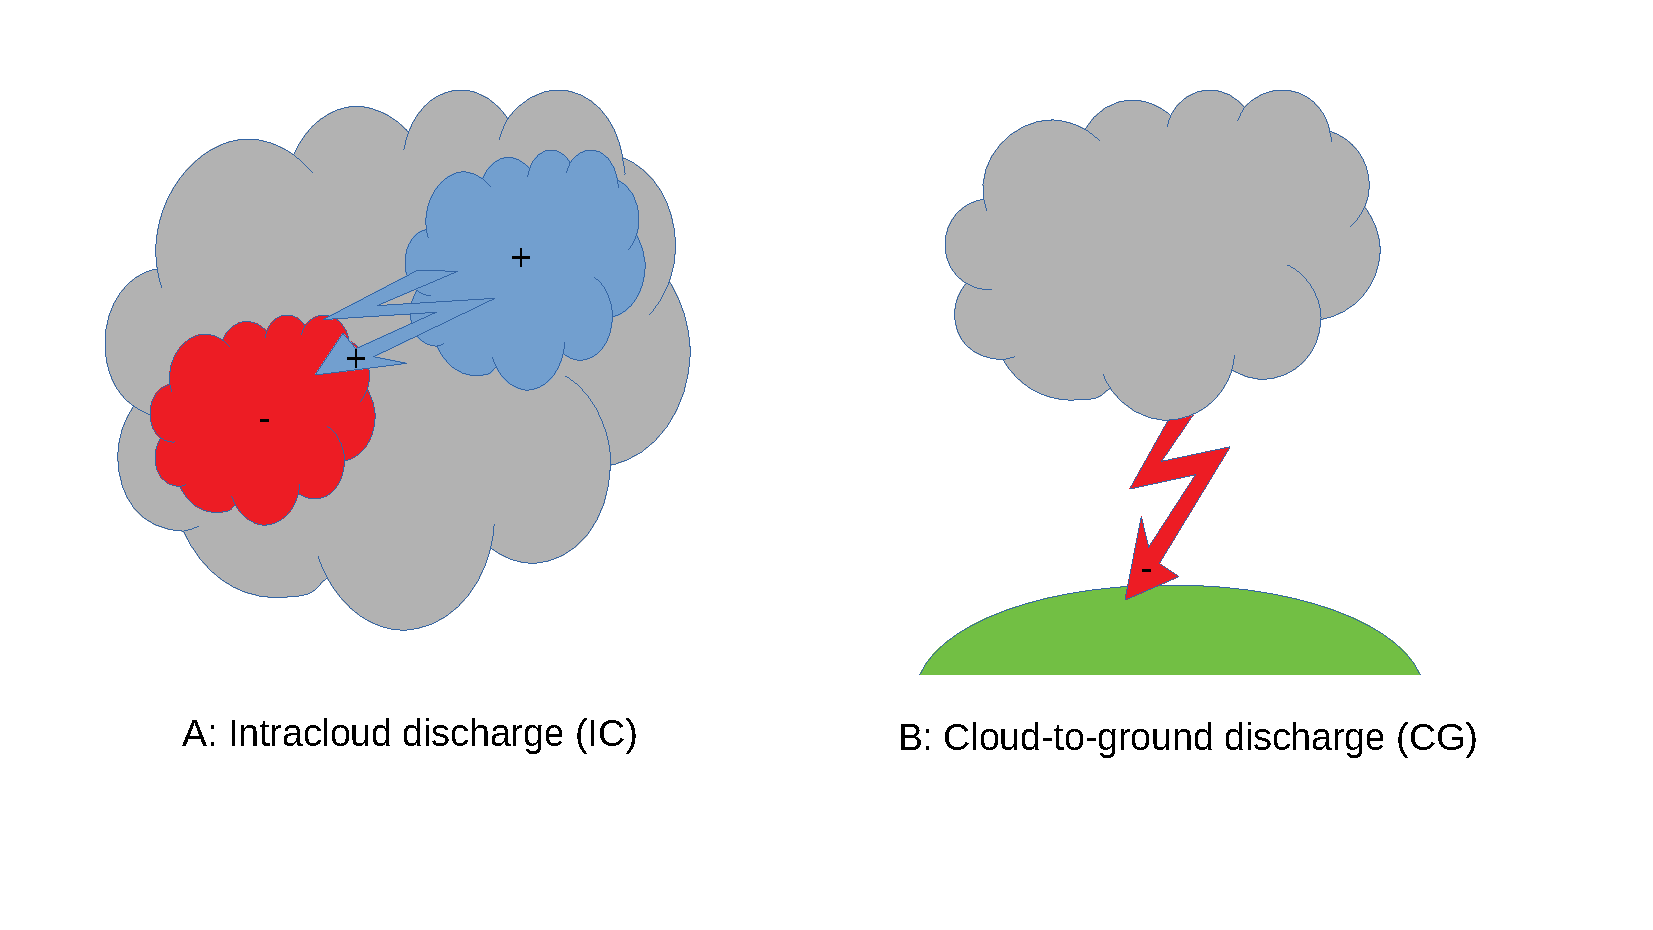
\includegraphics[width=\textwidth]{Figures/lyntyper.pdf}
    \caption{Simple diagram illustrating the two main categories of lightning. A shows an \acrfull{ic}, this could be between different storm cells or between different charge areas of the same storm cell. B shows a \acrfull{cg}, the polarity is defined by the charge change of earth. Negative cloud-to-ground (-CG) is defined by increase of negative charge at ground, and so positive cloud-to-ground (+CG) is defined by decrease of negative charge (increase in positive) at ground}
    \label{fig:lyntyper}
\end{figure}

\subsection{Winter lightning}
Winter lightning is a type of natural lightning specifically relevant to \acrshort{htl} in Norway, as discussed in the next section. It is a relatively well-studied phenomenon in Japan. Cold air from Siberia moves over the warm Tsushima current off the west coast of Japan, causing convection due to a strong temperature gradient between the cold air and the warm ocean. The supply of humidity from the seawater leads to formation of hydrometeors. The resulting convection has been shown to produce lightning strikes and thunderstorms during winter (\cite{michimoto2007}).

Winter lightning is also observed off the west coast of Norway (e.g \cite{march2016}; \cite{koeltzow2018}). Cold air is moved from the Arctic to the Norwegian coast where the ocean is warmed by the North Atlantic Current. The resulting temperature gradient gives rise to convection and subsequent electrification. As a result, there is a convective and electrically active belt along the coast of Norway during the winter, which is seen in the lightning climatology for winter in \cite{koeltzow2018}. Winter lightning also differs from summer lightning storms in that the frequency of lightning strikes is lower and the polarity is often more positive (\cite{michimoto2007}).
 
\section{Helicopter triggered lightning}
A \acrlong{htl} is thought to be triggered by the helicopter's presence, such that the required electric field for this to happen can be much smaller than for natural lightning. This also means that a system that would create an \acrshort{htl} may be hard to identify, as natural lightning needs not precede the \acrshort{htl}. 

Weather phenomena common to \acrshort{htl}-events are (from \cite{lande1999}):
\begin{itemize}
 \item \acrfull{oat} at flight level near freezing point 
 \item frozen precipitation, as snow, ice and graupel.
 \item inside of or directly below clouds.
 \item within 5 nautical miles of a Cumulonimbus cloud.
\end{itemize}

\begin{figure}
    \centering
    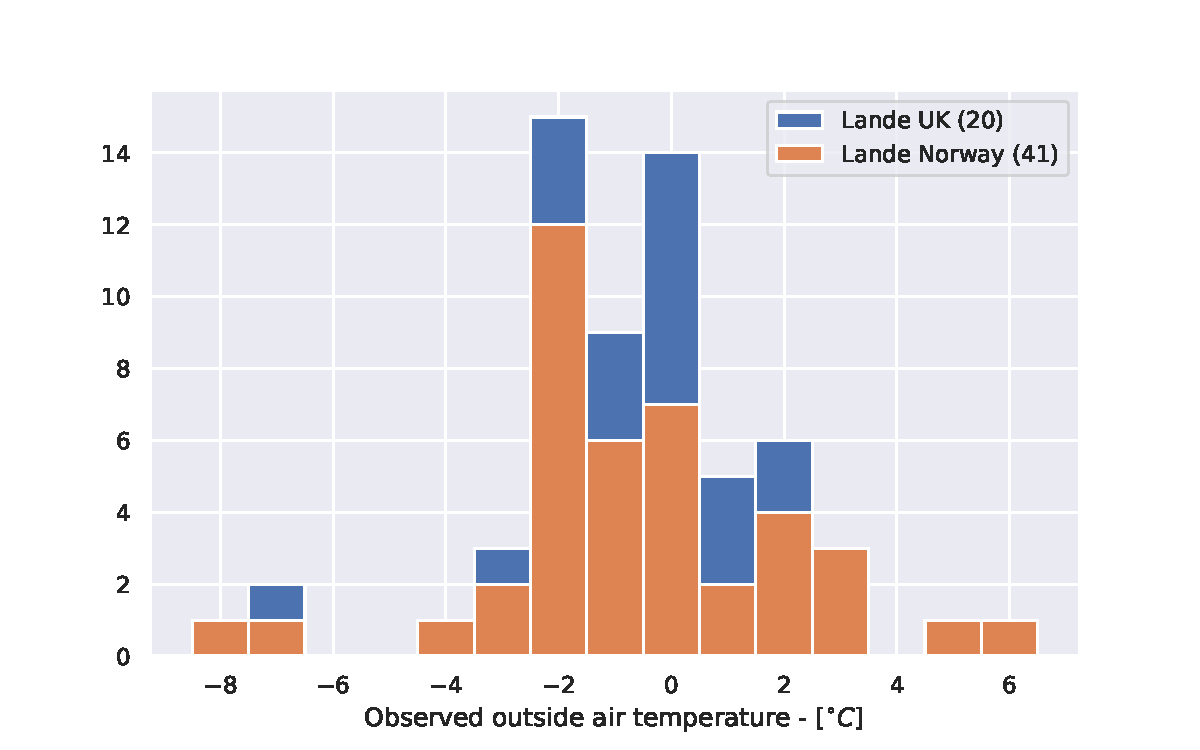
\includegraphics[width=\textwidth]{Figures/LandeTemp.pdf}
    \caption{Outside air temperature (\acrshort{oat}) adapted from earlier \acrshort{htl}-studies, showing the 0 and -2 degree temperatures to be most represented in \acrshort{htl}-cases} 
    \label{fig:landetemp}
\end{figure}

The phenomenon is thus believed to be caused by the helicopter entering or coming close to an electrically charged part of a convective system. This may be caused by several different mechanisms: The helicopter could be subject to a charge build-up during flight and then cause a discharge into the charged area of opposite polarity. However, given high enough charge density in the cloud, the charged area could also discharge into the helicopter \textit{without} charge buildup in the helicopter. Alternatively, the helicopter could induce a \acrshort{cg} by acting as part of the leader, see Figure \ref{fig:triggertyper}. 

A positively charged discharge is believed to cause more damage to helicopters than their negatively charged counterparts, as the action integral (Joule work\footnote{Any conductor has heat work (\textit{J}) based on the resistance (\textit{R}) and the current (\textit{I}) through the conductor: $J = I^2 R$} integrated over time, assuming $R = 1 \Omega$) of a positive lightning is higher than that of a negative lightning (\cite{hardwick1999}). The discharges to helicopters seem to also more often be positive (\cite{hardwick1999}).

\begin{figure}
    \centering
    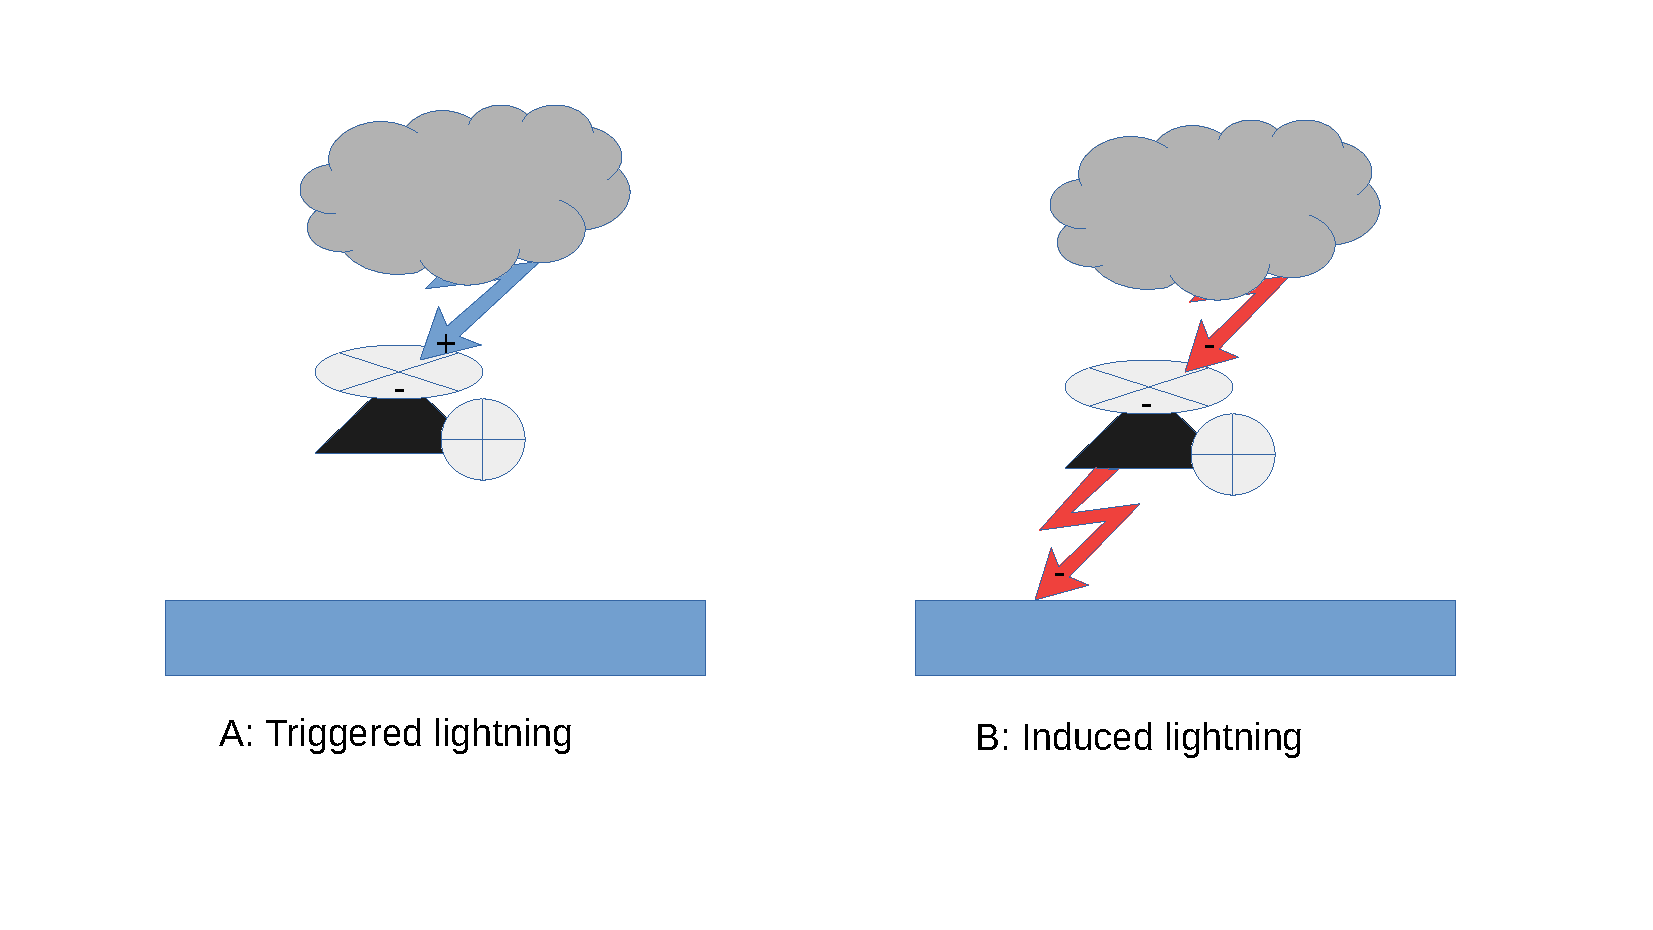
\includegraphics[width=\textwidth]{Figures/triggertyper.pdf}
    \caption{Illustration of different models for aircraft triggering. A shows the normal trigger situation, where the electrical discharge is grounded into the oppositely charged aircraft. B shows the situation where the aircraft is only acting as a pathway to the ground (Here ocean or land)}
    \label{fig:triggertyper}
\end{figure}

\section{Fixed wing triggered lightning}\label{sec:fwtl}

As introduced in Chapter \ref{ch:introduction}, a \acrfull{fwtl} is a similar phenomenon to \acrshort{htl}: lightning triggered instead by the presence of an airplane or a rocket. The main difference between \acrshort{fwtl} and \acrshort{htl} is that \acrshort{fwtl} is not solely a winter phenomenon; it occurs during all seasons \cite{uman2003}. Presumably, this is because planes fly higher and in a larger range of altitudes than helicopters: In summer, convective clouds can reach the tropopause, causing the electrical parts of the clouds to be spread further up, whilst in winter, the convection is not as deep, and the electrical parts of the clouds are closer to the surface (e.g. \cite{uman2003}; \cite{michimoto2007}).

\section{Helicopter trigger index}\label{sec:hti}
As stated in Chapter \ref{ch:introduction}, operational forecasting of \acrshort{htl} is relatively new. In Norway, the Norwegian Meteorological Institute began forecasting the risk of \acrshort{htl}, \acrfull{hti}, in 2016. The theory behind the forecast is based on findings by \cite{hardwick1999} and \cite{wilkinson2013}, and \acrshort{hti} is computed from four sub-indices, which are meteorological factors:
\begin{itemize}
    \item \textbf{Vertical wind speed} in the altitude that helicopters generally fly in.
    \begin{itemize}
        \item Computed from the maximum vertical wind speed within the 7 nearest grid cells in the forecasting model.
        \item Positive (upward) vertical wind gives a non-zero value, and negative (downward) vertical wind gives 0 value.
        \item Figure \ref{fig:vertical velocity} shows the conversion between vertical velocity in $m/s$ and this sub-index.
    \end{itemize}
    \item \textbf{Temperature} at the altitude that helicopters generally fly in.
    \begin{itemize}
        \item Temperatures in the $[0,-6] ^{\circ}C$ range gives non-zero value. 
        \item 0 for temperatures outside this range
        \item Figure \ref{fig:temperature} shows the conversion between temperature in $^{\circ}C$ and this sub-index.
    \end{itemize}
    \item \textbf{Total precipitation} during the last hour.
    \begin{itemize}
        \item Computed from the maximum precipitation within the 7 nearest grid cells in the forecasting model.
        \item Linear from $0\frac{mm}{hr}$ with 0 value to full value at $0.75\frac{mm}{hr}$ precipitation intensity.
        \item Figure \ref{fig:precipitation} shows the conversion between precipitation intensity in $mm/hr$ and this sub-index.
    \end{itemize}
    \item \textbf{Low clouds} in the surrounding area.
    \begin{itemize}
        \item Computed as the difference between the maximum and minimum cloud cover within the 7 nearest grid cells in the forecasting model. 
        \item Full cloud cover gives value 0, to exclude stratiform cloud systems and fog. No clouds also gives value 0. 
        \item Figure \ref{fig:cloud cover} shows the conversion between minimum and maximum cloud cover and this sub-index.
    \end{itemize} 
\end{itemize}

\begin{figure}
    \centering
    \begin{subfigure}{.45\textwidth}
    \centering
    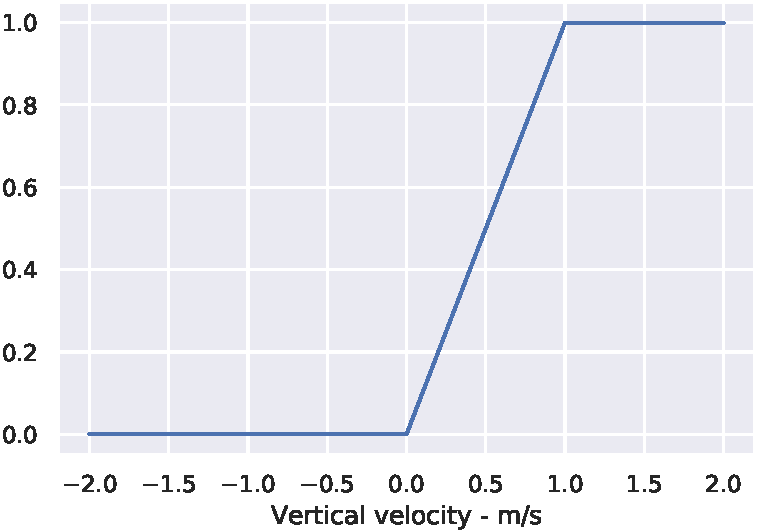
\includegraphics[width = \textwidth]{Figures/Wvar.pdf}
    \caption{Vertical velocity in meter per second}
    \label{fig:vertical velocity}
    \end{subfigure}
    \begin{subfigure}{.45\textwidth}
    \centering
    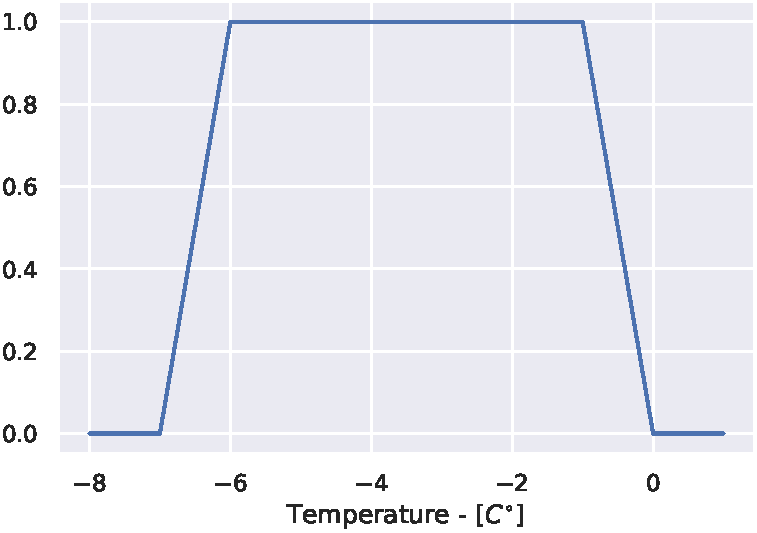
\includegraphics[width = \textwidth]{Figures/Tvar.pdf}
    \caption{Temperature in degrees celsius}
    \label{fig:temperature}
    \end{subfigure}
    
    \begin{subfigure}{.45\textwidth}
    \centering
    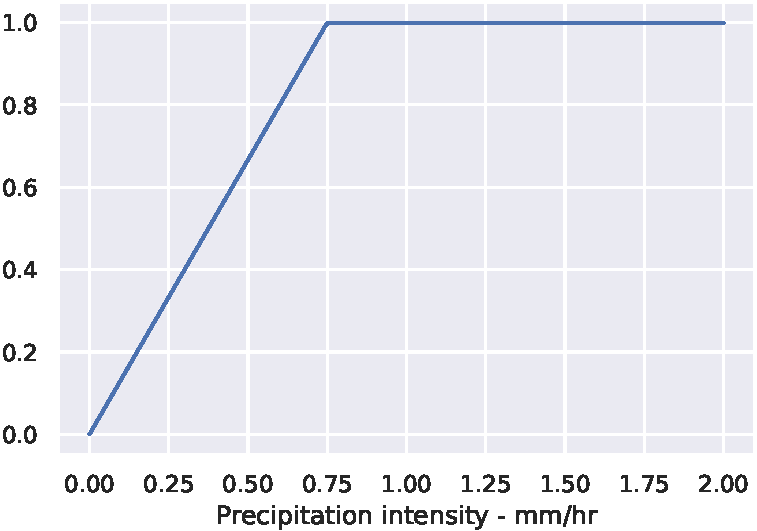
\includegraphics[width = \textwidth]{Figures/Pvar.pdf}
    \caption{Precipitation in mm/hr}
    \label{fig:precipitation}
    \end{subfigure}
    \begin{subfigure}{.45\textwidth}
    \centering
    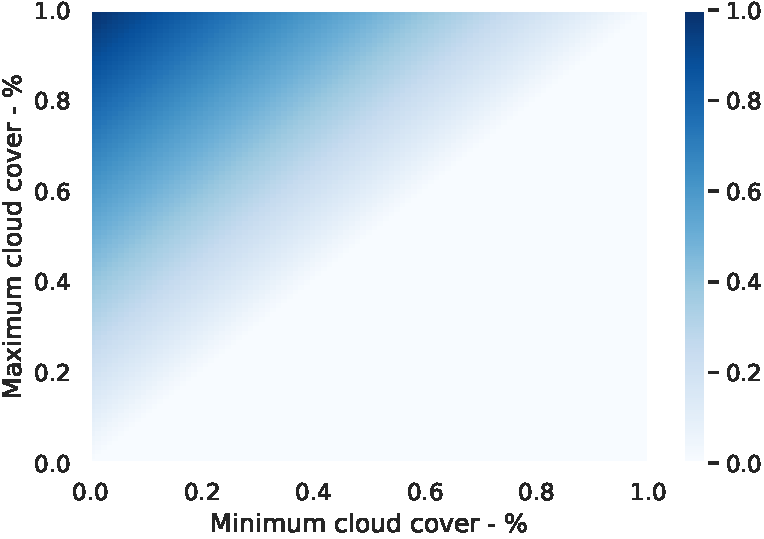
\includegraphics[width = \textwidth]{Figures/CCvar.pdf}
    \caption{Cloud cover maximum - cloud cover minimum in percentage}
    \label{fig:cloud cover}
    \end{subfigure}
    \caption{Sub-index value for different input for the four parameters used in the calculation of \acrshort{hti}}
    \label{fig:subindices}
\end{figure}

The \acrshort{hti} is the sum of these four sub-indices, \[\text{HTI} = \frac{\text{Vertical Wind}}{4} + \frac{\text{Temperature}}{4} + \frac{\text{Precipitation}}{4} +\frac{\text{Cloud}}{4}\] equally weighted, such that \acrshort{hti} is valued in the range $[0,1]$. The index is categorized in four different classes of severity, from no danger (White) to very high risk (Red). (See figure \ref{fig:hti}).
\begin{itemize}
    \item White: $HTI < 0.73$
    \item Yellow: $0.73 \leq HTI < 0.90 $
    \item Orange: $0.90 \leq HTI < 0.99 $
    \item Red: $0.99 \leq HTI $
\end{itemize}
The severity categories are based on discussion with the main offshore helicopter operators in Norway (Bristow and CHC), and are changed if deemed necessary after the yearly evaluation of the season. \acrshort{hti} is not based on a regression analysis, but rather a subjective review of the earlier cases of incidents.

\begin{figure}
    \centering
    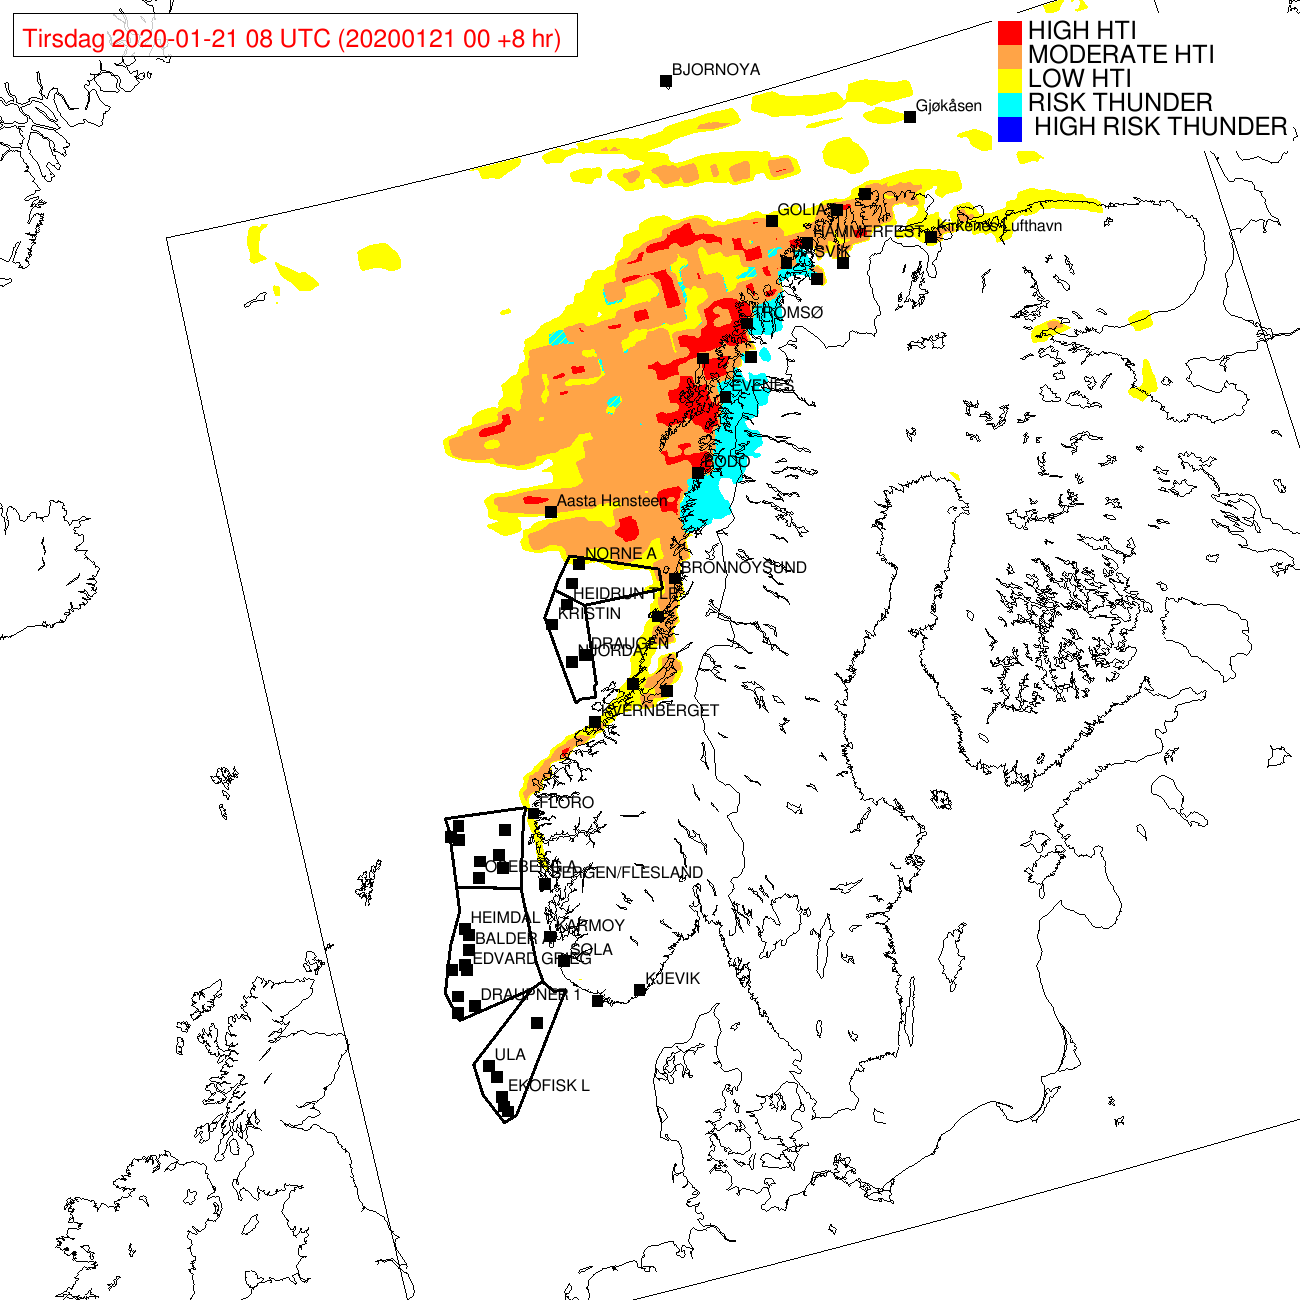
\includegraphics[width=\textwidth]{Figures/hti.png}
    \caption{Screenshot from https://www.ippc.no for 21. of January 2020, showing the HTI-forecast with 8 hour lead-time after midnight. The blue thunder-cells show another forecast-product from MET, forecasting risk for natural lightning. A plane was hit by lightning, and was therefore diverted from flying into Bodø during this forecasts valid time. }
    \label{fig:hti}
\end{figure}

